\documentclass[twocolumn,a4j]{jsarticle}
\setlength{\topmargin}{-20.4cm}
\setlength{\oddsidemargin}{-10.4mm}
\setlength{\evensidemargin}{-10.4mm}
\setlength{\textwidth}{18cm}
\setlength{\textheight}{26cm}

\usepackage[top=15truemm,bottom=20truemm,left=20truemm,right=20truemm]{geometry}
\usepackage[latin1]{inputenc}
\usepackage{amsmath}
\usepackage{amsfonts}
\usepackage{amssymb}
\usepackage[dvipdfmx]{graphicx}
\usepackage[hang,small,bf]{caption}
\usepackage[subrefformat=parens]{subcaption}
\usepackage[dvipdfmx]{color}
\usepackage{listings}
\usepackage{listings,jvlisting}
\usepackage{geometry}
\usepackage{framed}
\usepackage{color}
\usepackage[dvipdfmx]{hyperref}
\usepackage{ascmac}
\usepackage{enumerate}
\usepackage{tabularx}
\usepackage{cancel}
\usepackage{scalefnt}
\usepackage{overcite}
\usepackage{otf}
\usepackage{multicol}
\usepackage[geometry]{ifsym}

\renewcommand{\figurename}{Fig.}
\renewcommand{\tablename}{Table }

\lstset{
basicstyle={\ttfamily},
identifierstyle={\small},
commentstyle={\smallitshape},
keywordstyle={\small\bfseries},
ndkeywordstyle={\small},
stringstyle={\small\ttfamily},
frame={tb},
breaklines=true,
columns=[l]{fullflexible},
xrightmargin=0zw,
xleftmargin=3zw,
numberstyle={\scriptsize},
stepnumber=1,
numbersep=1zw,
lineskip=-0.5ex
}

% キャプション後ろのダブルコロンを消す
\makeatletter
\long\def\@makecaption#1#2{%
  \vskip\abovecaptionskip
  \iftdir\sbox\@tempboxa{#1\hskip1zw#2}%
    \else\sbox\@tempboxa{#1 #2}%
  \fi
  \ifdim \wd\@tempboxa >\hsize
    \iftdir #1\hskip1zw#2\relax\par
      \else #1 #2\relax\par\fi
  \else
    \global \@minipagefalse
    \hbox to\hsize{\hfil\box\@tempboxa\hfil}%
  \fi
  \vskip\belowcaptionskip}
\makeatother

% タイトル
\makeatletter
\def\@maketitle
{
\begin{center}
{\LARGE \@title \par}
\end{center}
\begin{flushright}
{\large \@date 報告書 No.28}\\
{\large M2 \@author}
\end{flushright}
\par\vskip 1.5em
}
\makeatother

\author{来代 勝胤}
\title{令和4年度 6月 第1週 報告書}
\date{2022/6/6}

\begin{document}
\columnseprule=0.1mm
\maketitle

\section*{報告内容}
\begin{enumerate}[1.]
  \item 枚数差の組み合わせ変更
  \item 粒子像の重ね合わせ
  \item 来週の予定
\end{enumerate}

\section{枚数差の組み合わせ変更}
共同研究報告の際に,
渦中心の主流方向速度が遅くなることや,
タイヤ周り流れの解析において,
範囲ごとに対応枚数を変更する必要があることがわかった.
そのため,三角翼後流の撮影結果について,
枚数差を変更してPTVを適用した.
また,計算状の対応枚数差 $n$ は後流速度 $u'$ が主流速度 $u = 250\;[\mathrm{mm/s}]$ と同等の場合,
LLS間隔 $\Delta x = 2.5\;[\mathrm{mm}]$およびフレームレート $f = 800\;[1/s]$ の関係から,
以下の式により求められる.
\begin{eqnarray*}
  n = \frac{\Delta x}{u \times f} = 8.0\;[枚]\\
\end{eqnarray*}

\subsection*{PTVの適用結果}

\begin{figure}[htbp]
  \footnotesize
  \begin{center}
    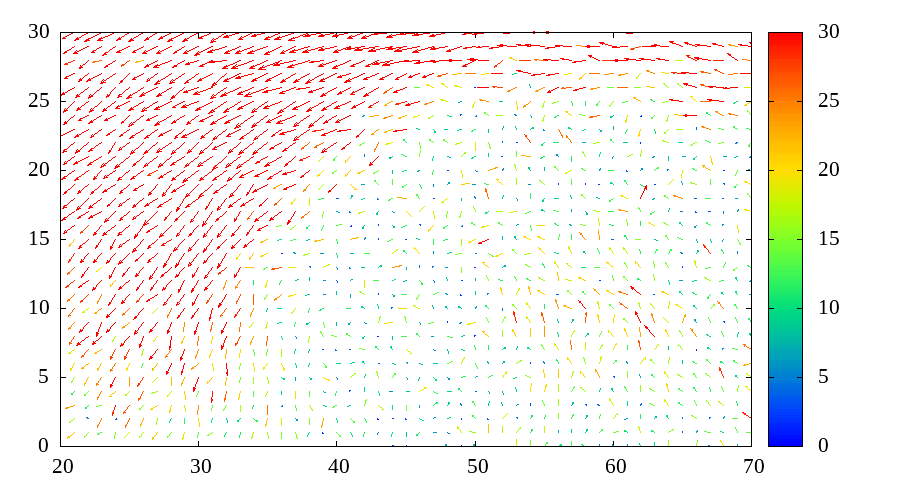
\includegraphics[width=80mm]{../images/velocity_n=8.png}
    \caption{Velocity vectors : n = 8}
    \vskip \baselineskip
    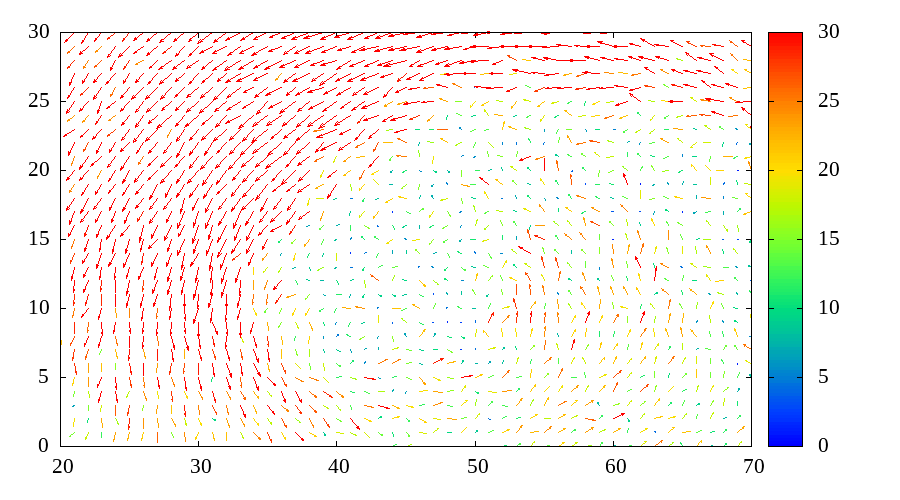
\includegraphics[width=80mm]{../images/velocity_n=9.png}
    \caption{Velocity vectors : n = 9}
  \end{center}
\end{figure}

\newpage
また,対応枚数差 $n$ から,後流速度 $u'$ は以下の式により求められる.
\begin{eqnarray*}
  u' = \frac{\Delta x}{n \times f}\; [\mathrm{mm/s}]
\end{eqnarray*}
PTVの適用結果をみると,$n$ が増加するにしたがって
渦の範囲が狭まり,中心の流れが鮮明化することがわかる.
この結果より,(1)渦中心の主流方向速度が低下すること,
(2) 流れの場所ごとにPTVを適用することの有効性 を
示すことができた.

\begin{figure}[htbp]
  \footnotesize
  \begin{center}
    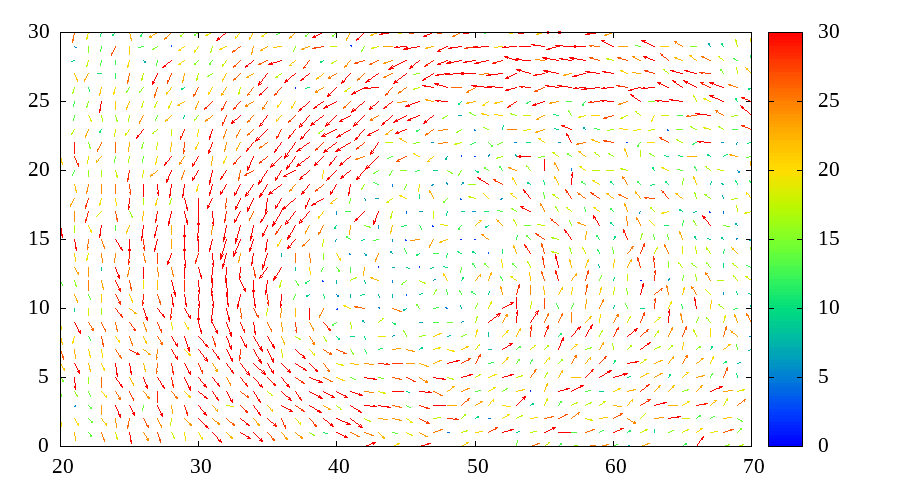
\includegraphics[width=80mm]{../images/velocity_n=10.png}
    \caption{Velocity vectors : n = 10}
    \vskip \baselineskip
    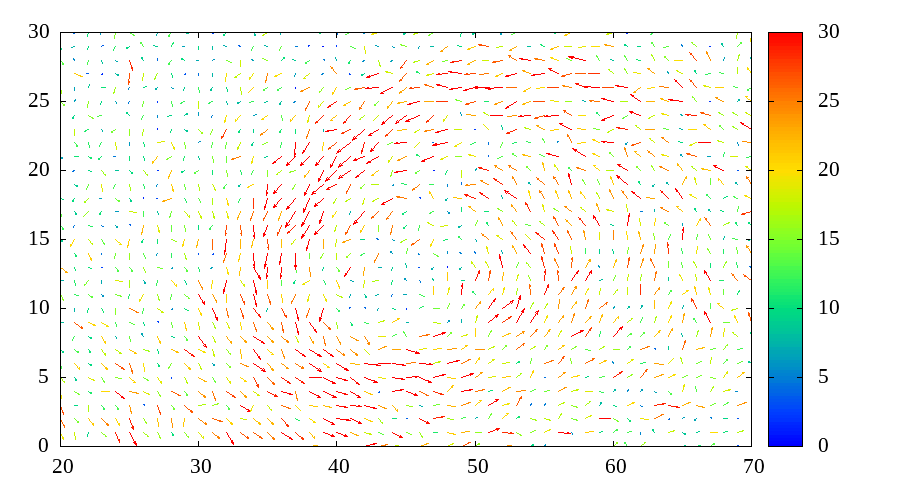
\includegraphics[width=80mm]{../images/velocity_n=11.png}
    \caption{Velocity vectors : n = 11}
    \vskip \baselineskip
    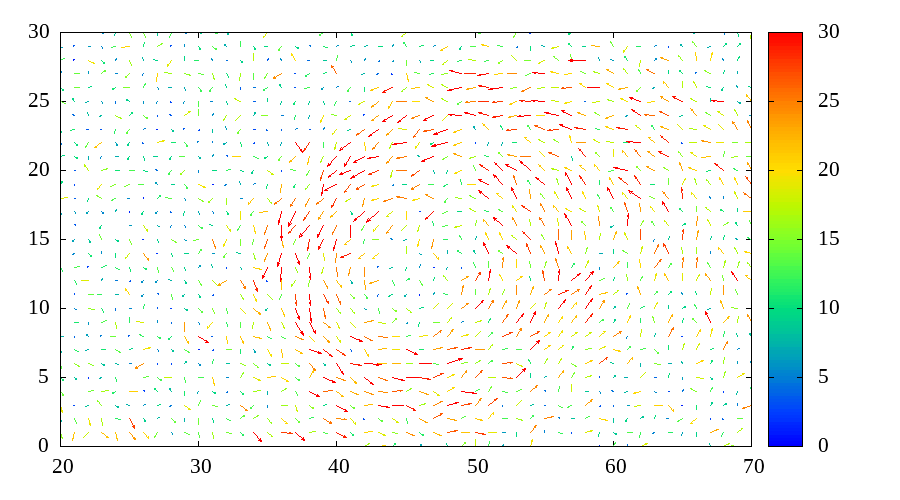
\includegraphics[width=80mm]{../images/velocity_n=12.png}
    \caption{Velocity vectors : n = 12}
  \end{center}
\end{figure}

\begin{figure}[htbp]
  \footnotesize
  \begin{center}
    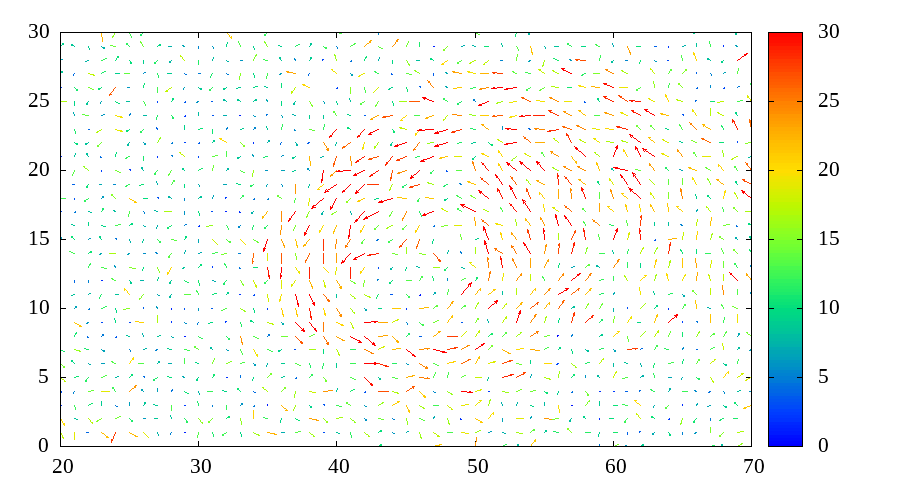
\includegraphics[width=80mm]{../images/velocity_n=13.png}
    \caption{Velocity vectors : n = 13}
    \vskip \baselineskip
    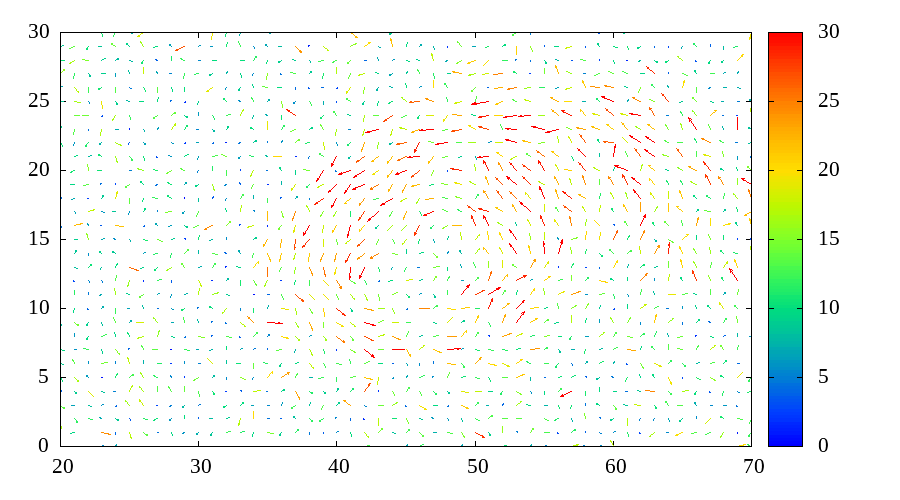
\includegraphics[width=80mm]{../images/velocity_n=14.png}
    \caption{Velocity vectors : n = 14}
    \vskip \baselineskip
    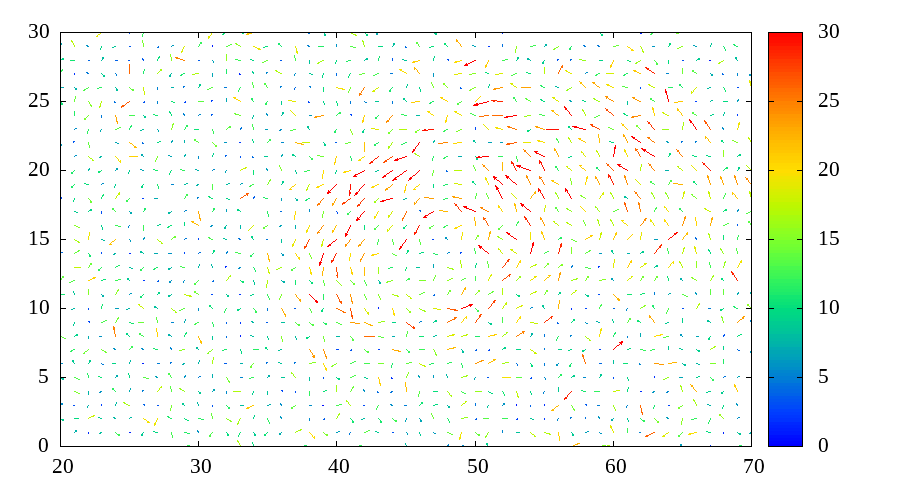
\includegraphics[width=80mm]{../images/velocity_n=15.png}
    \caption{Velocity vectors : n = 15}
    \vskip \baselineskip
    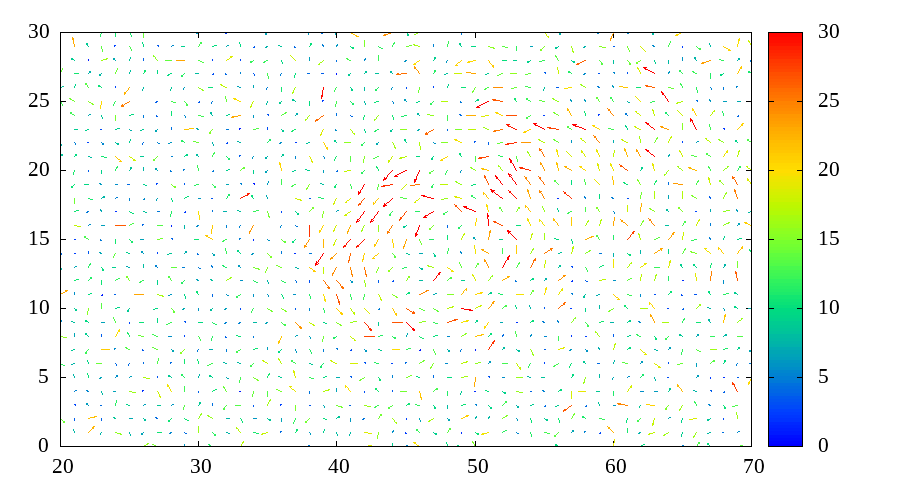
\includegraphics[width=80mm]{../images/velocity_n=16.png}
    \caption{Velocity vectors : n = 16}
  \end{center}
\end{figure}

\newpage

\section{粒子像の重ね合わせ}
時間変動を記録するために
速度ベクトルを増やす必要がある.
そこで,画像の重ね合わせを行って
疑似的に粒子数を増加させ解析を行った.\\

\subsection{画像の生成}

\begin{figure}[htbp]
  \footnotesize
  \begin{center}
    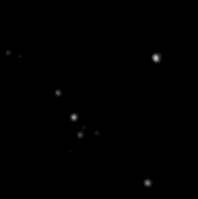
\includegraphics[width=80mm]{../images/blue.bmp}
    \caption{Particles image of blue : not overlapped}
    \includegraphics[width=80mm]{../images/blue_overlap.bmp}
    \caption{Particles image of blue : overlapped 3 sheets}
  \end{center}
\end{figure}

\subsection{PTVの適用結果}
\begin{figure}[htbp]
  \footnotesize
  \begin{center}
    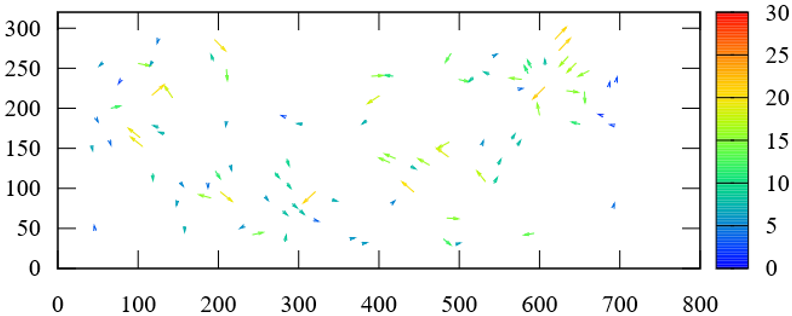
\includegraphics[width=85mm]{../images/vector.png}
    \caption{Vectors : not overlapped}
    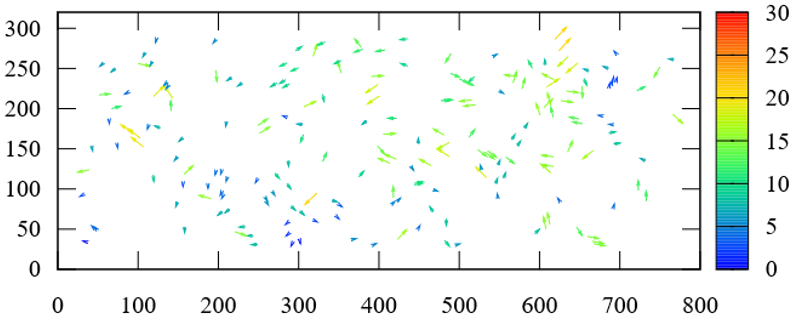
\includegraphics[width=85mm]{../images/vector_overlap.png}
    \caption{Vectors : overlapped 3 sheets}
  \end{center}
\end{figure}
\section{来週の予定}
\begin{itemize}
  \item 数値シミュレーション結果のグラフ作成
  \item ISTP-33 原稿作成
\end{itemize}

\end{document}